\begin{appendices}
\counterwithin{figure}{section}
\section{Results of optimisation flags}\label{apdx:opt-flags}

\begin{figure}[H]
\centering
\begin{minipage}{0.45\textwidth}
\begin{tikzpicture}[scale=0.65]
\begin{axis}[
	title={\textbf{Number of solver nodes}},
	ylabel={Number of solver nodes},
	%ymode=log,
	xlabel={Parameter file},
	x label style={yshift=-0.5cm},
	xtick={2,4,6,8,10,12,14,16},
	xticklabels={2_2,3_5,4_7,5_9,6_11,7_14,8_15,9_16},
	x tick label style={rotate=90, anchor=east},
	ymajorgrids=true,
	xmajorgrids=true,
	legend pos=north west,
	cycle list name=color list,
	]

\addplot+[mark=*] coordinates {
(2,0) (4,0) (6,113) (8,512) (10,11671) (12,51492) (14,327718) (16,546476) };
\addlegendentry{-O0}

\addplot+[mark=*] coordinates {
(2,0) (4,0) (6,0) (8,267) (10,7052) (12,44769) (14,328143) (16,547184)};
\addlegendentry{-O1}

\addplot+[mark=*] coordinates {
(2,0) (4,0) (6,0) (8,267) (10,7052) (12,44769) (14,328143) (16,547184)};
\addlegendentry{-O2}

\addplot+[mark=*] coordinates {
(2,0) (4,0) (6,0) (8,267) (10,6622) (12,44769) (14,328143) (16,547184) };
\addlegendentry{-O3}

\end{axis}

\end{tikzpicture}
\end{minipage}
%
\begin{minipage}{0.45\textwidth}
\begin{tikzpicture}[scale=0.65]
\begin{axis}[
	title={\textbf{Time taken}},
	ylabel={Time taken in seconds},
	%ymode=log,
	xlabel={Parameter file},
	x label style={yshift=-0.5cm},
	xtick={2,4,6,8,10,12,14,16},
	xticklabels={2_2,3_5,4_7,5_9,6_11,7_14,8_15,9_16},
	x tick label style={rotate=90, anchor=east},
	ymajorgrids=true,
	xmajorgrids=true,
	legend pos=north west,
	cycle list name=color list,
	]

\addplot+[mark=*] coordinates {
(2,0.002527) (4,0.008836) (6,0.030193) (8,0.052777) (10,0.662101) (12,1.94038) (14,11.2637) (16,19.0305)};
\addlegendentry{-O0}

\addplot+[mark=*] coordinates {
(2,0.000509) (4,0.002246) (6,0.007113) (8,0.02607) (10,0.199171) (12,1.07673) (14,6.14513) (16,10.2163)};
\addlegendentry{-O1}

\addplot+[mark=*] coordinates {
(2,0.000139) (4,0.000923) (6,0.001386) (8,0.00733) (10,0.095159) (12,0.529529) (14,3.19886) (16,5.32569)};
\addlegendentry{-O2}

\addplot+[mark=*] coordinates {
(2,1e-06) (4,0.000428) (6,0.001355) (8,0.008099) (10,0.097074) (12,0.565429) (14,3.57982) (16,5.7996)};
\addlegendentry{-O3}

\end{axis}
\end{tikzpicture}
\end{minipage}
\caption{Optimisations with initial model on problem files \textit{without} solutions}
\end{figure}

\vspace{0.5cm}

\begin{figure}[H]
\centering
\begin{minipage}{0.45\textwidth}
\begin{tikzpicture}[scale=0.65]
\begin{axis}[
	title={\textbf{Number of solver nodes}},
	ylabel={Number of solver nodes},
	%ymode=log,
	xlabel={Parameter file},
	x label style={yshift=-0.5cm},
	xtick={1,3,5,7,9,11,13,15,17},
	xticklabels={1_1, 2_3, 3_6, 4_8, 5_10, 6_12, 7_15, 8_16, 9_17},
	x tick label style={rotate=90, anchor=east},
	ymajorgrids=true,
	xmajorgrids=true,
	legend pos=north west,
	cycle list name=color list,
	]

\addplot+[mark=*] coordinates {
(1,1) (3,1) (5,19) (7,266) (9,1313) (11,16198) (13,5755) (15,49723) (17,88077) };
\addlegendentry{-O0}

\addplot+[mark=*] coordinates {
(1,1) (3,1) (5,19) (7,1) (9,615) (11,13737) (13,1) (15,48055) (17,85000)};
\addlegendentry{-O1}

\addplot+[mark=*] coordinates {
(1,1) (3,1) (5,19) (7,1) (9,615) (11,13737) (13,1) (15,48055) (17,85000)};
\addlegendentry{-O2}

\addplot+[mark=*] coordinates {
(1,1) (3,1) (5,19) (7,1) (9,615) (11,13737) (13,1) (15,48055) (17,85000) };
\addlegendentry{-O3}

\end{axis}

\end{tikzpicture}
\end{minipage}
%
\begin{minipage}{0.45\textwidth}
\begin{tikzpicture}[scale=0.65]
\begin{axis}[
	title={\textbf{Time taken}},
	ylabel={Time taken in seconds},
	%ymode=log,
	xlabel={Parameter file},
	x label style={yshift=-0.5cm},
	xtick={1,3,5,7,9,11,13,15,17},
	xticklabels={1_1, 2_3, 3_6, 4_8, 5_10, 6_12, 7_15, 8_16, 9_17},
	x tick label style={rotate=90, anchor=east},
	ymajorgrids=true,
	xmajorgrids=true,
	legend pos=north west,
	cycle list name=color list,
	]

\addplot+[mark=*] coordinates {
(1,0.031298) (3,0.032611) (5,0.050352) (7,0.061549) (9,0.097533) (11,0.811384) (13,0.693712) (15,2.54343) (17,4.24591)
};
\addlegendentry{-O0}

\addplot+[mark=*] coordinates {
(1,0.033393) (3,0.033572) (5,0.037248) (7,0.047957) (9,0.064181) (11,0.367553) (13,0.075426) (15,1.39464) (17,2.4274)};
\addlegendentry{-O1}

\addplot+[mark=*] coordinates {
(1,0.029873) (3,0.033931) (5,0.037498) (7,0.034361) (9,0.048934) (11,0.339495) (13,0.033142) (15,1.10833) (17,1.91377)};
\addlegendentry{-O2}

\addplot+[mark=*] coordinates {
(1,0.030431) (3,0.033729) (5,0.036896) (7,0.033898) (9,0.051484) (11,0.329233) (13,0.033632) (15,1.11276) (17,1.90869)};
\addlegendentry{-O3}

\end{axis}
\end{tikzpicture}
\end{minipage}
\caption{Optimisations with improved model on problem files \textit{with} solutions}
\end{figure}

\vspace{0.5cm}

\begin{figure}[H]
\centering
\begin{minipage}{0.45\textwidth}
\begin{tikzpicture}[scale=0.65]
\begin{axis}[
	title={\textbf{Number of solver nodes}},
	ylabel={Number of solver nodes},
	%ymode=log,
	xlabel={Parameter file},
	x label style={yshift=-0.5cm},
	xtick={2,4,6,8,10,12,14,16},
	xticklabels={2_2,3_5,4_7,5_9,6_11,7_14,8_15,9_16},
	x tick label style={rotate=90, anchor=east},
	ymajorgrids=true,
	xmajorgrids=true,
	legend pos=north west,
	cycle list name=color list,
	]

\addplot+[mark=*] coordinates {
(2,0) (4,0) (6,113) (8,512) (10,8257) (12,2675) (14,18960) (16,30705) };
\addlegendentry{-O0}

\addplot+[mark=*] coordinates {
(2,0) (4,0) (6,0) (8,267) (10,6786) (12,0) (14,18169) (16,29331)};
\addlegendentry{-O1}

\addplot+[mark=*] coordinates {
(2,0) (4,0) (6,0) (8,267) (10,6786) (12,0) (14,18169) (16,29331)};
\addlegendentry{-O2}

\addplot+[mark=*] coordinates {
(2,0) (4,0) (6,0) (8,267) (10,6786) (12,0) (14,18169) (16,29331) };
\addlegendentry{-O3}

\end{axis}

\end{tikzpicture}
\end{minipage}
%
\begin{minipage}{0.45\textwidth}
\begin{tikzpicture}[scale=0.65]
\begin{axis}[
	title={\textbf{Time taken}},
	ylabel={Time taken in seconds},
	%ymode=log,
	xlabel={Parameter file},
	x label style={yshift=-0.5cm},
	xtick={2,4,6,8,10,12,14,16},
	xticklabels={2_2,3_5,4_7,5_9,6_11,7_14,8_15,9_16},
	x tick label style={rotate=90, anchor=east},
	ymajorgrids=true,
	xmajorgrids=true,
	legend pos=north west,
	cycle list name=color list,
	]

\addplot+[mark=*] coordinates {
(2,0.001865) (4,0.007652) (6,0.025196) (8,0.041011) (10,0.379043) (12,0.388171) (14,0.93558) (16,1.34073)
};
\addlegendentry{-O0}

\addplot+[mark=*] coordinates {
(2,0.000863) (4,0.001497) (6,0.003385) (8,0.021171) (10,0.163485) (12,0.031769) (14,0.37022) (16,0.558146)};
\addlegendentry{-O1}

\addplot+[mark=*] coordinates {
(2,0.000551) (4,0.00099) (6,0.001367) (8,0.011141) (10,0.139455) (12,0.003976) (14,0.266379) (16,0.431757)};
\addlegendentry{-O2}

\addplot+[mark=*] coordinates {
(2,0.000111) (4,0.0) (6,0.001373) (8,0.013258) (10,0.140305) (12,0.004111) (14,0.270614) (16,0.421794)};
\addlegendentry{-O3}

\end{axis}
\end{tikzpicture}
\end{minipage}
\caption{Optimisations with improved model on problem files \textit{without} solutions}
\end{figure}



\section{b}

\begin{figure}[H]
\centering
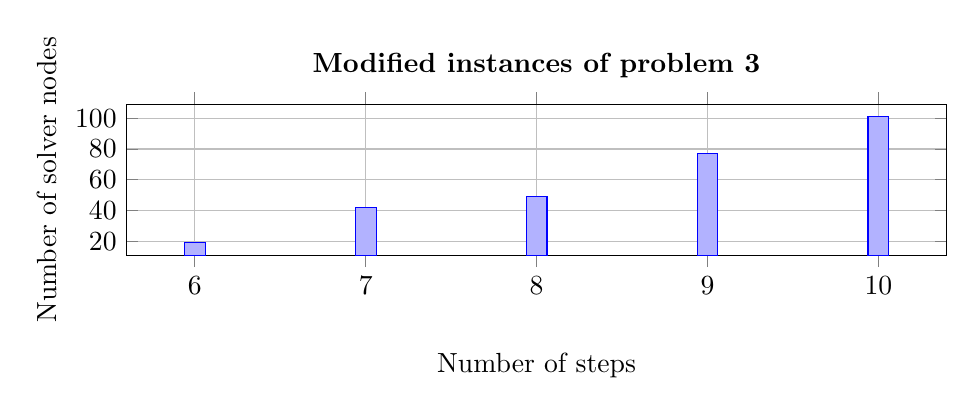
\begin{tikzpicture}
\begin{axis}[
	title={\textbf{Modified instances of problem 3}},
	ybar,
	bar width=0.75em,
	width=12cm,
	height=3.5cm,
	ylabel={Number of solver nodes},
	%ymode=log,
	xlabel={Number of steps},
	x label style={yshift=-0.5cm},
	symbolic x coords={6,7,8,9,10},
	xtick=data,
	%x tick label style={rotate=90, anchor=east},
	ymajorgrids=true,
	xmajorgrids=true,
	legend pos=outer north east,
]
\addplot
coordinates {
(6,19) (7,42) (8,49) (9,77) (10,101) 
};
\end{axis}
\end{tikzpicture}
\n
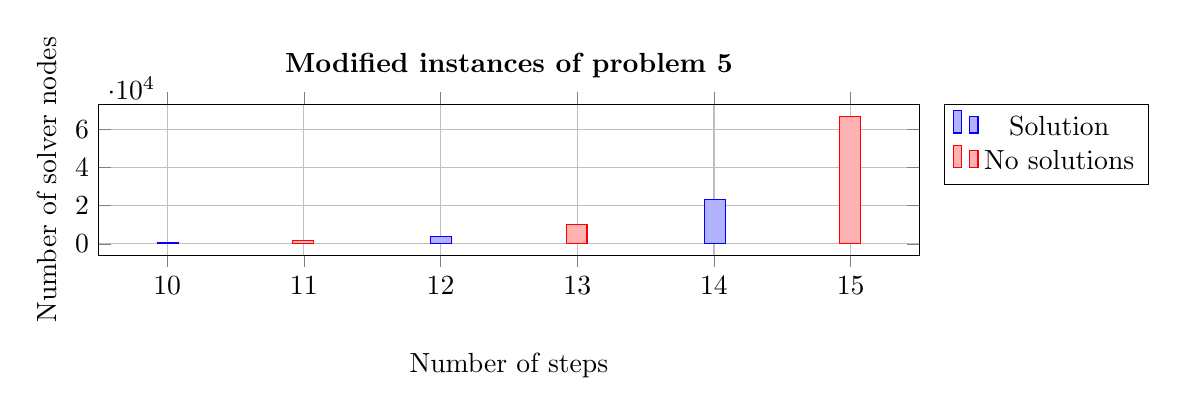
\begin{tikzpicture}
\begin{axis}[
	title={\textbf{Modified instances of problem 5}},
	ybar,
	bar width=0.75em,
	width=12cm,
	height=3.5cm,
	ylabel={Number of solver nodes},
	%ymode=log,
	xlabel={Number of steps},
	x label style={yshift=-0.5cm},
	symbolic x coords={10,11,12,13,14,15},
	%x tick label style={rotate=90, anchor=east},
	ymajorgrids=true,
	xmajorgrids=true,
	legend pos=outer north east,
]

\addplot+[
	xshift=0.5em,
	legend image post style={xshift=-0.5em}	
]
coordinates {
(10,615) (12,3617) (14,23315)
};
\addlegendentry{Solution}

\addplot+[
	xshift=-0.5em,
	legend image post style={xshift=0.5em}	
]
coordinates {
(11,1611) (13,10278) (15,66518)
};
\addlegendentry{No solutions}

\end{axis}
\end{tikzpicture}
\caption{b1}
\end{figure}

\end{appendices}
